%%%%%%%%%%%%%%%%%%%%%%%%%%%%%%%%%%%%%%%%%%%%%%%%%%%%%%%%%%%
% EPFL report package, main thesis file
% Goal: provide formatting for theses and project reports
% Author: Mathias Payer <mathias.payer@epfl.ch>
%
% This work may be distributed and/or modified under the
% conditions of the LaTeX Project Public License, either version 1.3
% of this license or (at your option) any later version.
% The latest version oset ft?f this license is in
%   http://www.latex-project.org/lppl.txt
%
%%%%%%%%%%%%%%%%%%%%%%%%%%%%%%%%%%%%%%%%%%%%%%%%%%%%%%%%%%%
\documentclass[a4paper,11pt,oneside]{report}
% Options: MScThesis, BScThesis, MScProject, BScProject
\usepackage[BScThesis,lablogo]{EPFLreport}
\usepackage{xspace}
\usepackage{listings}
\usepackage{xcolor}


\definecolor{codegreen}{rgb}{0,0.6,0}
\definecolor{codegray}{rgb}{0.5,0.5,0.5}
\definecolor{codepurple}{rgb}{0.58,0,0.82}
\definecolor{backcolour}{rgb}{0.95,0.95,0.92}

\lstdefinestyle{mystyle}{
    backgroundcolor=\color{backcolour},   
    commentstyle=\color{codegreen},
    keywordstyle=\color{magenta},
    numberstyle=\tiny\color{codegray},
    stringstyle=\color{codepurple},
    basicstyle=\ttfamily\footnotesize,
    breakatwhitespace=false,         
    breaklines=true,                 
    captionpos=b,                    
    keepspaces=true,                 
    numbers=left,                    
    numbersep=5pt,                  
    showspaces=false,                
    showstringspaces=false,
    showtabs=false,                  
    tabsize=2
}

\lstset{style=mystyle}

\title{Retrofitting defences to C++ code}
\author{Hassan Habib}
\supervisor{Nicolas Badoux}
\adviser{Prof. Dr. sc. ETH Mathias Payer}
%\coadviser{Second Adviser}
%\expert{The External Reviewer}

\newcommand{\sysname}{Retrowrite\xspace}
\newcommand{\todobox}[3]{%
    \colorbox{#1}{\textcolor{white}{\sffamily\bfseries\scriptsize #2}}%
    ~\textcolor{blue}{#3} %
    \textcolor{#1}{$\triangleleft$}%
}
\newcommand{\nb}[1]{\todobox{orange}{Nicolas:}{#1}}

\begin{document}
\maketitle
%\makededication
%\makeacks

\begin{abstract}
The \sysname project is a static binary rewriter that allows to audit \nb{whaty
do ou mean by audit?} programs where the
source code is not available.
\textit{C++} being a largelly \nb{grammar pass pls!} used programming language, we must ensure that
progams written in this language are safe. 

Our task is to test \sysname on various \nb{speak more globally about C++ packages} \textit{Debian} packages to see if the
binary could be modified for instrumetation.

From our results, we can see that \sysname worked on a lot \nb{quantify} of packages but in
too many cases, the assembly obtained could not be compiled back to a
functionning executable. Also, only a few programs encountered runtime errors.
We concluded that there is still works to do to have a fully \textit{C++} support.

\end{abstract}


\maketoc

%%%%%%%%%%%%%%%%%%%%%%
\chapter{Introduction}
%%%%%%%%%%%%%%%%%%%%%%

The introduction is a longer writeup that gently eases the reader into your
thesis~\cite{dinesh20oakland}. Use the first paragraph to discuss the setting.
In the second paragraph you can introduce the main challenge that you see.
The third paragraph lists why related work is insufficient.
The fourth and fifth paragraphs discuss your approach and why it is needed.
The sixth paragraph will introduce your thesis statement. Think how you can
distill the essence of your thesis into a single sentence.
The seventh paragraph will highlight some of your results
The eights paragraph discusses your core contribution.

This section is usually 3-5 pages.

%%%%%%%%%%%%%%%%%%%%
\chapter{Background}
%%%%%%%%%%%%%%%%%%%%
In this section, we will give a some backround \nb{pass your check
through a spell checker e.g., grammarly} in order to understand
the experience \nb{the experience is a bit vague. Be clearer in that you want to
build up knowledge for later.}

\section{Compiler}
Computer programs can be executed in two different ways: they can be interpreted
by a software (an interpreter) or they can be compiled into machine code that can
then be executed by the hardware. 


In the first approach, the interpreter will read each line it encounters, and
then it will translate them and run them one at a time. Interpreting a program
is much slower than running the machine code generated by a compiler \nb{an
explanantion why would be greaet: you have to run the interpreted next to it!}.

In the second approach, a compiler is needed to translate the source code into binary code.
The compiler will analyze all the source code and generate the machine code.
Note that it will not execute the source code but only generate an executable
file.
\nb{Maybe add a paragraph on why we still use interepreted language: easier to port between systems for example. Higher level -> easier to write}
We will now discuss the most common format of binary executable.


\section{Binary executable}
\subsection{ELF format}
%source man page elf
%
The dominant executable format for binary in Unix system is the ELF\footnote{Executable
and Linkable Format} format. 

An executable file respecting the ELF format must follow a certain layout. At
first, it must have an ELF header followed by a program header table or a section
header table, or both. 
The ELF header contains the offset \nb{to}of the section header table and the program
header table. The program header contains information about the segments used
at runtime. The section header table \nb{one word too much}lets locate all the single sections of the
binary. Figure ~\ref{fig:elf} illustrates the structure of an ELF file. The
\textit{readelf}~\cite{readelfMan} command in \textit{GNU/Linux}
allows us to see the different section's information.

\begin{figure}[h]
    \centering
    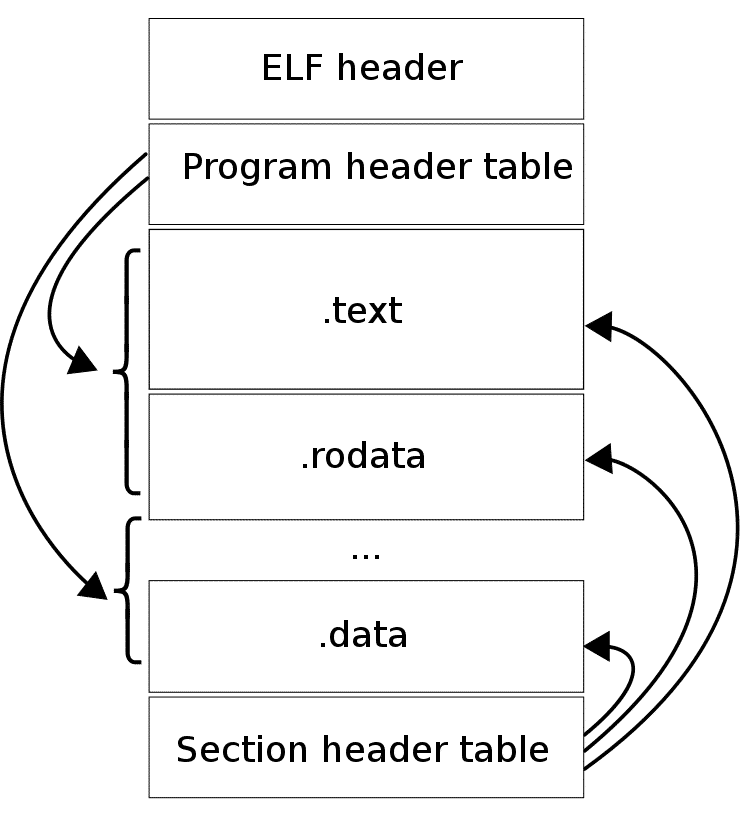
\includegraphics[width=8cm]{elf_structure.png} 
    \caption{Structure of ELF file}
    \label{fig:elf}
\end{figure}

\nb{Much better background until now, good job!}


\subsection{Usage}
The binary executable \nb{produced}given by the compiler can now be used to run the program.
Having the program in this new file does not remove the utility of the source code.
Indeed, a compiler can be executed with multiple flags in order to have a more 
specific executable. For example, a program might need to be tested before its release.
To do so, memory errors can be discovered using a feedback-guided fuzzer
combined with sanitization.
To check the memory, a tool named \textit{Address Sanitizer} (ASan)~\cite{ASan}
can be used by compiling the source code with a certain flag \nb{and what does
this flag do? -> add instrumentation!}.
In the case of an end user wanting to test a closed source software, it is
nearly impossible to get the program compiled with the instrumentation needed.
Tools such as binary rewriters can be used in order to face this issue.


\section{Binary rewritting}
%%Pourquoi c'est important ???
Binary rewritting consists of modifying an executable in the absence of while
maintaining functionnality. It can be used for multiple reasons as for example
for program optimization, program obfuscation or as in the case of \sysname for
security policy enforcement via instrumentation. 


Binary rewriters can be divided into two main approaches: dynamic
instrumetation and static instrumentation.

\subsection{Dynamic instrumentation}
%%executer virtuellement le programe
In this scheme, the rewritting is done while the program is executed. Usually
the binary is executed side by side with the rewriter engine. In order to
analyze and interact with the program during the execution. The rewriter might
use the OS's primitves as the PTRACE API in Linux for example.  An advantage of
dynamic instrumentation is that analyzing the whole binary might be avoided.
This is practical for large binaries. However, the disadvantage of using this
technique is the high performance cost. Translating the program at runtime does
not come with no cost and the overhead is way higher than running a modified
binary executable~\cite{dinesh20oakland}.


\subsection{Static instrumentation}
Contrary to dynamic instrumentation, static rewriters operates on binaries
stored in persistent \nb{at static time } memory. It outputs a new binary
executable that corresponds to the initial executable but rewritten. This
generated executable have the advantage of being almost as fast as the original
executable that would have been compiled for instrumentation as the overhead
introduced are usually low.


\subsection{Steps in binary rewritting}
Both dynamic and static instrumentation follow four main steps:
\begin{enumerate}
    \item Parsing:
        This step consist of obtaining the instruction stream from the binary
        and pass it to a disassembler.
    \item Analysis:
        This part consists of gaining as much information as possible. The
        objectif is to recover the structure of the source code.
    \item Transformation:
        Here, we must find all the locations where instrumentation must be
        added or removed. 
    \item Code generation:
        We have to make sure that adding the instrumentation does not modify the
        behaviour of the executable. The modified executable must be sound.
        There are multiple techniques for this part. \nb{Code gen is
            mostly going back from the lifted language (AR; dissabled  instructions)
        to machine code again. }
\end{enumerate}
%\begin{figure}[h]
%    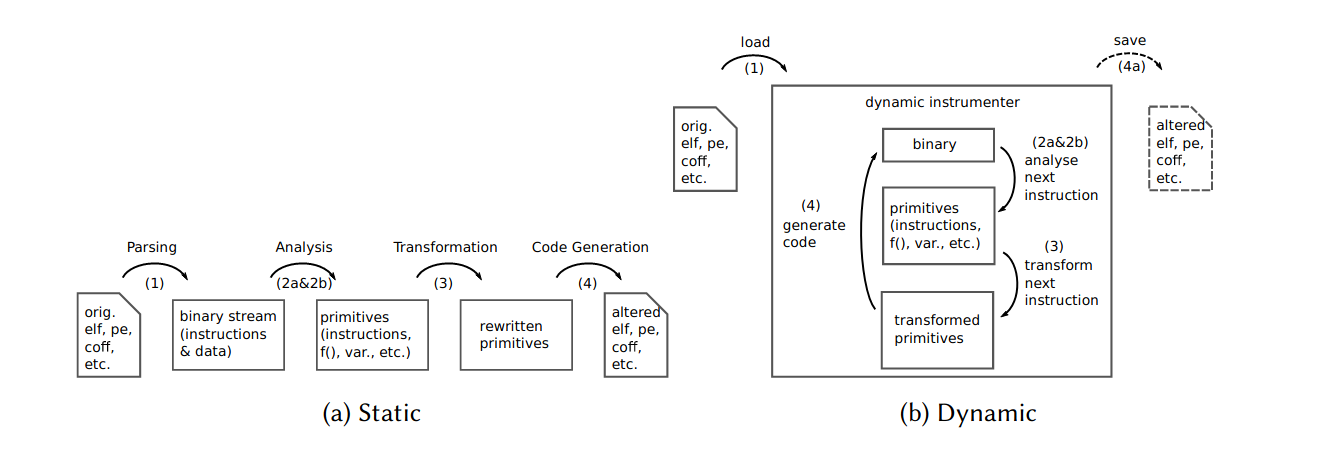
\includegraphics[width=\linewidth]{required_steps.png} 
%    \caption{Required steps for binary rewritting\nb{Make two figures. Add
%            refernce to the figure in the text. The figure shold help understand
%    something and not just be there for beauty}}
%    \label{fig:steps}
%\end{figure}
\subsection{Transformation and Code genreation techniques}
There are multiples techniques for the transformation and code generation
parts. The simplest technique is called \textit{Trampoline}. All new code are
added in new sections in the binary. Branches are then added to redirect to the
right location after an instrumentation point. In this technique, no reference
or branches are broken. \nb{Why do we need to do that. Eplain the challenge of
fixed refernec earlier.}

Another technique is named \textit{Direct}. This is one of the oldest
technique. Here the code is simply overwritten. We have to make sure to reajust
every branch and references\nb{and is hard? why?}.


The technique used by \sysname is called \textit{Symbolization}. It
consists of transforming the binary into an assembly text file. It transforms
all references constants into assembly labels. Then, many tools can insert
instrumentation into the reassembled file. Unlike the trampoline technique,
this method is defined as being \textit{zero-overhead} \nb{why? Speak about the
overhead in each section!}
%add example of symbolization

\section{Retrowrite}
%link to paper
Retrowrite~\cite{dinesh20oakland} is a binary rewriter developped by HexHive.
It uses the symbolization technique by generating re-assembleable assembly.
Retrowrite has as objectif to be sound. \nb{why it is sound ?} It uses
\textit{Capstone} as a disassembler and \textit{pyelftools} as a binary parser.

\section{Other security techniques}
\textit{C/C++} are \nb{two}one of the most used programming languages. They are
mainly\nb{used} for their runtime performance and low level memory access \nb{capabilities}, but this
comes with a cost. In this language\nb{C or C++}, memory and type safety are managed by the
programmers. Tools can be used to enforce the safety of software. For example,
one might want to use \textit{HexType} to enforce type safety.
\subsection{HexType}
\textit{HexType} is a tool written by the \textit{HexHive} lab in order to
detect type confusion in software written in \textit{C++}. Typecast are
normally checked statically. This can lead to type confusion as no one prevents
the program to cast an object of incompatible base type. \textit{HexType}
remedy to this issue by transforming static checks to runtime checks.


%%%%%%%%%%%%%%%%
\chapter{Goal}
%%%%%%%%%%%%%%%%
As stated in their paper~\cite{dinesh20oakland}, \textit{Retrowrite} was
firstly designed to support Linux x86-64 PIC binaries that were written in the
\textit{C Programming Language}. The main obstacle for adding support for
\textit{C++} is that \nb{remove word}the symbolization of C++ exception
handlers is not yet supported. Multiple works were done in order to add support
for C++ as it can be seen in the \textit{Retrowrite} repository
~\cite{gitCommit}.

\nb{Discuss what was the status when you started the
project. Why is it interesting etc...}


\nb{We are missing a page about challenges. This should be much longer.}

\section{Challenges}
At the beginning of the academic year, \sysname did not support C++ yet. 

\section{Task}
The task was to test many packages from the
\textit{Debian}~\cite{debian} distribution. Debian being a widely used
distribution, we thought it would be a good idea to use it as a source. 
We tested Retrowrite on a bunch of programs that can be found on Debian.
The test were not extensive as we were only testing if the command
\textit{--help} worked. The purpose of the testing was to see if the compiler
was able to compile the assembly file generated by \sysname.
Then we chose some programs where we try to run \sysname on them, and we try to
see where exactly the program crashes.

\nb{This whole paragraph
    should be part of the above one where you gently explain why we need more
    testing and why we wanted to test on this code (diversity of C++ coding patterns
for example). and why not Chromium (too big, not handled by Rretrowrite)}


%%%%%%%%%%%%%%%%%%%%%%%%
\chapter{Implementation}
%%%%%%%%%%%%%%%%%%%%%%%%

The main script is \textit{clone.sh}. It will start several containers which will
each take care of one package. This script also takes care of running the
command that will prepare the results.

\section{Docker}
The first decision was to test \textit{Retrowrite} in
\textit{docker}~\cite{merkel2014docker} containers. This allows us to emulate
\textit{Debian} on any machine. Each container will execute
\textit{entrypoint.sh} on a specific package. The binaries available from the
command \textit{apt install}~\cite{apt} are stripped, so we had to download the
source code and compile the program ourselves. Then we ran the program with the
argument "\textit{--help}" and compared the exit code with the recompiled
program from the assembly file re-assambled by retrowrite. The programs are
then sorted according to their output code.


\section{Linking}
One problem encountered was recompiling the
assembly files by linking them to the correct shared-libraries. To do so, a 
script was written called  \textit{flib.sh} which takes as argument the original binary
file. It will then return, using the command "ldd"\cite{ldd} the list of
libraries to link. 

\section{List of packages}

Having obtained a list of packages from the Debian distribution
\cite{sourcePackage}, we needed a way of filtering to only obtain
a list of packages written in \textit{C++}. To do this, we use the script
\textit{filter\_c++\_packages.sh}. It will simply look in the information given
in \textit{apt show}~\cite{apt} if the package was written in \textit{C++} or
not. 

\section{Filtering the result}
When the docker containers have finished executing their commands, the
\textit{result\_count.sh} script will be executed. This script takes care of searching
and sorting the results by arranging them and putting them in a new folder.
%explain the categories when it is more clear

\section{Use of exceptions}
We also needed a way to find which binaries were using exception. We noticed
that all binary files using exceptions also had a call instruction to
\verb|__cxa_begin_catch@plt| function or
\verb|__cxa_allocate_exception@plt|, both in the plt section.
So we just looked in the \textit{.rela.plt} section and search for the
\verb|__cxa_allocate_exception| symbol. The script is named \textit{elfexceptions.py}


%\section{Three programs}
%We have chosen three programs that we will test manually and try to find out
%where the errors may come from. They were selected from the top starred project
%in GitHub in order to have programs that are used by a large amount of people.
%The three programs are flameshot~\cite{flameshot}, bitcoind~\cite{bitcoind} and
%fish-shell~\cite{fish}.


All the scripts used can be found in the GitHub
\href{https://github.com/ha2san/debian_docker/tree/main/scripts}{repository}~\cite{repo}.

%%%%%%%%%%%%%%%%%%%
\chapter{Evaluation}
%%%%%%%%%%%%%%%%%%%
\nb{better use autoref}
In figure ~\ref{fig:popular}, you can see the result of our scripts on the most
popular pacakges in \textit{Debian}. The figure ~\ref{fig:remaining}
corresponds to the remaining packages found in other list. You can read the
exact numbers in table ~\ref{table:popular} and ~\ref{table:remaining}\nb{ref
not working}. The
\textit{discard} line corresponds to the packages where the program was not
testable. Running them with \textit{--help} leads to a crash or an error. 
The category "\textit{unsuccessful compilation}" means that we were not able to
compile the re-assembled assembly back to an executable for various reason as
missing shared-libraries or the assembly file contains some error. It was not
possible to categorize these errors as \textit{clang} always outputs the same
error in each situation: "\textit{<unknown>:0: error: Undefined temporary symbol .L26312
}". The "\textit{runtime error}" category corresponds to when we succeed to run
the modified executable but a segmentation fault was encountered.

\nb{Be careful in the figure that everything is readable}
\begin{figure}[h]
    \centering
    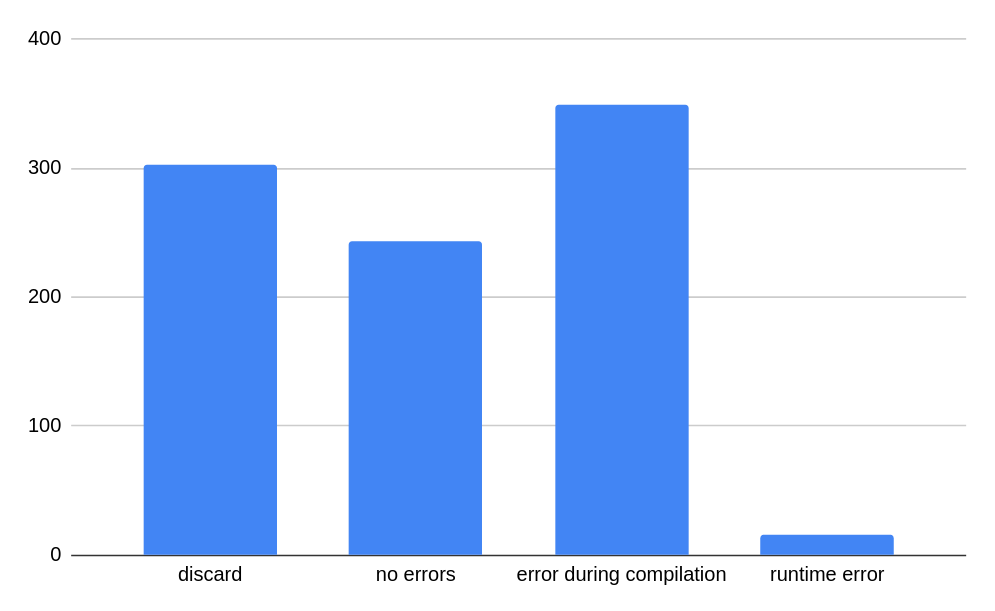
\includegraphics[width=15cm]{popular_packages.png} 
    \caption{\sysname on popular packages}
    \label{fig:popular}
\end{figure}

\begin{figure}[h]
    \centering
    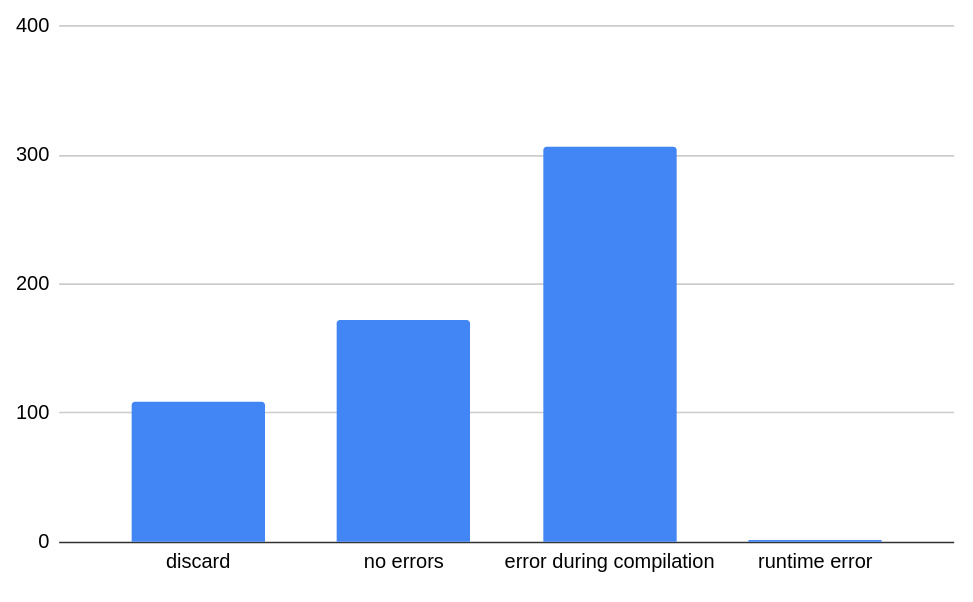
\includegraphics[width=15cm]{remaining_packages.png} 
    \caption{\sysname on remaining packages}
    \label{fig:remaining}
\end{figure}

\begin{table}[h]
    \centering
    \label{table:popular}
    \begin{tabular}{ll}
        \hline
        category                & \#packages \\
        \hline
        discard                  & 302  \\
        no errors                & 243  \\
        unsuccessful compilation & 349  \\
        runtime error            & 16   \\
        total                    & 910  \\ 
        \hline
    \end{tabular}
    \caption{Popular packages}
\end{table}


\begin{table}[h]
    \centering
    \label{table:remaining}
    \begin{tabular}{ll}
        \hline
        category                & \#packages \\
        \hline
        discard                  & 109  \\
        no crash                 & 172  \\
        unsuccessful compilation & 306  \\
        runtime error            & 2    \\
        total                    & 589  \\
        \hline
    \end{tabular}
    \caption{Remaining packages}
\end{table}

As you can see in thes figures, the most dominant category is the
"\textit{unsuccessful compilation}" one. Only a few programs crashed during the
runtime. This is a nice result as \sysname claims that the code produce is
sound.

By reading the \sysname paper~\cite{dinesh20oakland}, we understand that
the biggest issue with adding \textit{C++} support was to handle symbolization
of exception handlers. It seems that is not yet fully supported as testing a
simple program using exception leads to a runtim error:

\lstinputlisting[language=C++]{exception.cpp}

Retrowrite succeeded to rewrite the executable but running it leads to a segmentation fault.
We wanted to see for all the packages, which one fails and was using
exceptions. The result can be seen in figure ~\ref{fig:exception} and
~\ref{table:exception}.

As you can see, most of the segmentation fault were encountered with programs
using exception. The difference is not that big, but we see that the compilation
was more successful when the program was using exceptions. We understant from
the test done that the program crahses only if he gets in a catch clause.

\newpage

\begin{figure}[h]
    \centering
    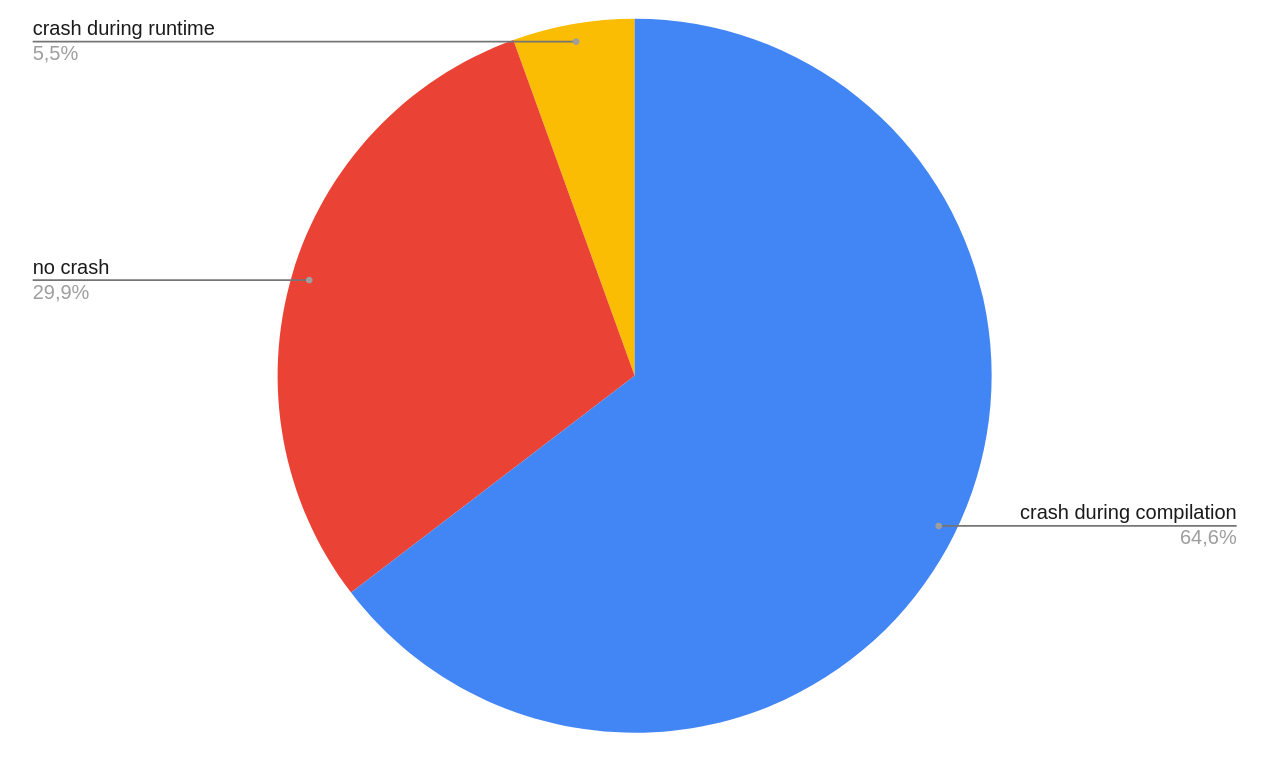
\includegraphics[width=15cm]{exception.png} 
    \caption{Packages using exceptions}
    \label{fig:exception}
\end{figure}

\begin{table}[h]
    \centering
    \begin{tabular}{ll} 
        \hline
        category                & \#packages  \\ 
        \hline
        crash during compilation & 199         \\
        no crash                 & 92          \\
        crash during runtime     & 17          \\
        \hline
    \end{tabular}
    \caption{Packages using exception}
    \label{table:exception}
\end{table}

\newpage
\begin{figure}[h]
    \centering
    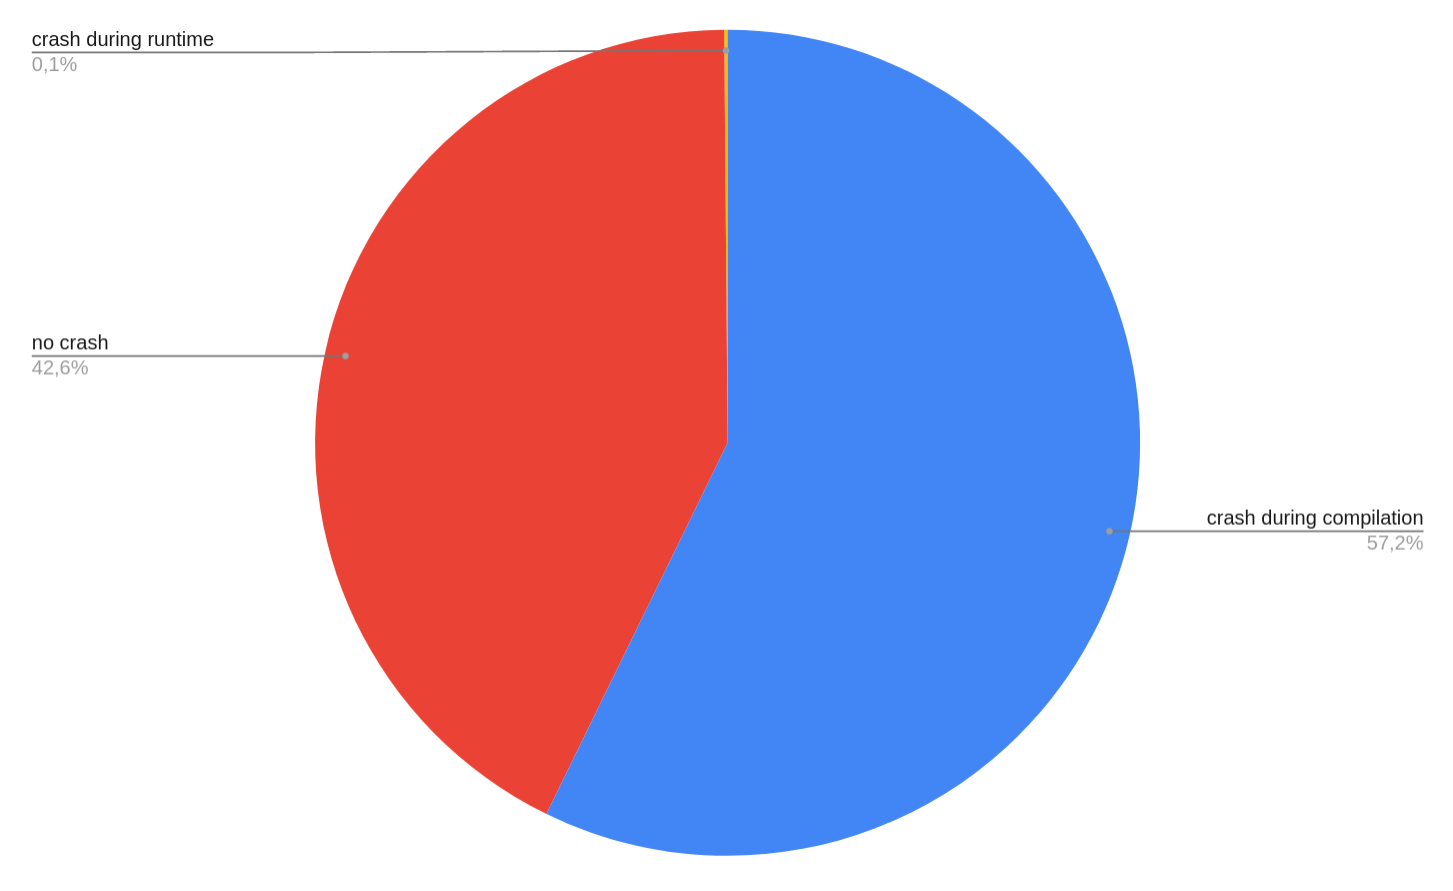
\includegraphics[width=15cm]{no_exception.png} 
    \caption{Packages not using exceptions}
    \label{fig:no_exception}
\end{figure}

\begin{table}[h]
    \centering
    \begin{tabular}{ll} 
        \hline
        category                & \#packages  \\ 
        \hline
        crash during compilation & 427         \\
        no crash                 & 318         \\
        crash during runtime     & 1           \\
        \hline
    \end{tabular}
    \caption{Packages not using exceptions}
\end{table}


%%%%%%%%%%%%%%%%%%%%%%%
%\chapter{Related Work}
%%%%%%%%%%%%%%%%%%%%%%%
%
%I can cite other rewritter.



%%%%%%%%%%%%%%%%%%%%
\chapter{Conclusion}
%%%%%%%%%%%%%%%%%%%%

In general, \sysname worked on a lot of packages, and we encountered few runtime
errors. The main problem was that it was not possible to compile the
re-assembled assembly back on most of the packages. The results also showed
that \sysname can not hanlde exceptions yet. And we had to find the
shared-libraries ourselves. It would be an enhancement if retrowrite could to
it for x86 CPU as it seems that this option is only available for \textit{ARM}
cpu~\cite{retroArm}.

\cleardoublepage
\phantomsection
\addcontentsline{toc}{chapter}{Bibliography}
\printbibliography

% Appendices are optional
% \appendix
% %%%%%%%%%%%%%%%%%%%%%%%%%%%%%%%%%%%%%%
% \chapter{How to make a transmogrifier}
% %%%%%%%%%%%%%%%%%%%%%%%%%%%%%%%%%%%%%%
%
% In case you ever need an (optional) appendix.
%
% You need the following items:
% \begin{itemize}
% \item A box
% \item Crayons
% \item A self-aware 5-year old
% \end{itemize}

\end{document}
